\chapter{System Architecture}
\label{architecture}
\thispagestyle{empty}

\begin{quotation}
{\footnotesize
\noindent{\emph{``Morty: I mean, why would a Pop-Tart want to live inside a toaster, Rick? I mean, that would be like the scariest place for them to live. You know what I mean?\\
Rick: You're missing the point Morty. Why would he drive a smaller toaster with wheels? I mean, does your car look like a smaller version of your house? No. ''}}
\begin{flushright}
Rick and Morty (Season 1, Episode 4)
\end{flushright}
}
\end{quotation}



\vspace{0.5cm}

The framework implements three layers: hierarchical core, computational graph, and the blocks. The implementation details of these layers and of other utility functions are presented in this chapter. Figure \ref{fig:overall} illustrates the architecture of the system.

The framework exploits \texttt{mushroom}~\cite{mushroom}, a reinforcement learning library of AI\&R Lab of Politecnico di Milano, which provides learning algorithms, features, environments, policies, distributions and function approximators. Apart from the methods implemented, our framework adopts some of the design concepts of the \texttt{mushroom} library. Datasets are formed with the same structure, that is, every step is represented with a tuple containing state, action, reward, next state, and the absorbing and last step flags. In addition, the hierarchical core is indeed a hierarchical version of mushroom core. Our framework is implemented to be compatible with any flat reinforcement learning mushroom algorithm.

\section{Hierarchical Core}
Hierarchical core unit is developed as an interface between the diagram and Python. A computational graph is passed to the hierarchical core in the declaration. The hierarchical core contains the methods to run it with a requested amount of steps or episodes. In the beginning of each run the hierarchical core initiates the computational graph and at the end of the runs calls it to stop. The runs can be made for the hierarchical algorithm to learn or to evaluate its performance. During the learning runs, policies of blocks with a learning algorithm in the computational graph are updated. A flag is passed to the computational graph to signal the mode of the run. 

\begin{figure}[t!]
      \centering
      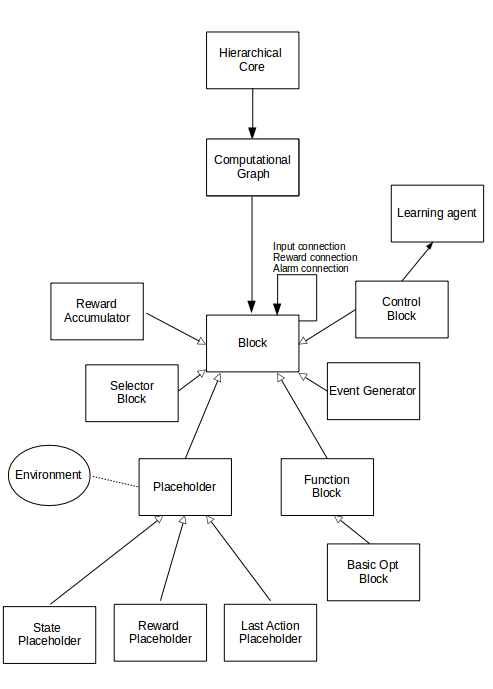
\includegraphics[width = \textwidth]{./pictures/overall_new.png}
      \caption{System architecture}
      \label{fig:overall}
\end{figure}

\section{Computational Graph}
Computational graph establishes the connection between the environment and the block diagram. In the declaration, it receives a list of blocks and a model. 

When the computational graph calls a block, it sends a request to that block to activate its functionality. To call a block, computational graph checks the input, reward and alarm connections of that block. The last outputs of the input connection blocks are passed in an input list. A block can have one reward connection at most. The last output of the reward connection block, if exists, is passed as a reward. The alarm output of the alarm connections are passed as alarms. If a block does not have an alarm connection, it should wake up at each state. Thus, a default alarm is passed in such cases. Finally, in order to indicate the blocks whether or not they should update their policy, a learn flag is passed.

Computational graph calls the blocks in the sorted list one by one until the cycle completes. Each cycle corresponds to a step of the environment. 
At the start of each episode, the computational graph takes the initial state of the environment, and all the blocks are called for a reset. The first primitive control action, that is the last output of the last block in the sorted block list, is stored in the last action placeholder. Computational graph starts each cycle by applying the primitive control action to the environment. Then, the computational graph observes the response of the environment in the form of a state and reward data. The state and reward data are passed to the corresponding placeholders. The state of the environment can be absorbing due to success or failure which results to terminate the episode. Another reason for a step to be the last of the current episode is that the environment horizon is reached. Two variables that signal the last and the absorbing states of the environment are passed to the blocks by the computational diagram when they are called.

In order to activate the blocks in the correct order, computational graph needs them to be sorted in accordance with their connections, using a topological sort algorithm. To achieve this, the block diagram is described as a directed graph where each node is a block and the edges are the connections between them. Placeholders are not considered during the construction of the graph. This is because, as described previously in chapter~\ref{proposed}, placeholders are not called as the other block objects. They are employed to pass the environment data to the rest of the graph. Thus, regardless of their connections, they ought to be the first ones in the list. In fact, placeholders do not need to have a connection as their input connection is the environment itself and the environment is not a part of the block diagram. Therefore, they are not declared as nodes and thus no edges are created between any other blocks and placeholders. Additionally, the blocks that are members of the block lists inside the selector blocks are not included in the block list passed to the computational graph. These blocks retrieve their inputs through the selector block. However, their reward connections are independent of the selector block. To maintain the integrity of the topological sort, while constructing the graph for sorting, connections of these blocks are represented as the connections to the selector block. 
This graph is sorted with a function already implemented in the \texttt{networkx} library. The sorted block list that the computational graph uses is a concatenated list of placeholders and the blocks sorted with the above-mentioned algorithm.
Computational graph calls the blocks also to initialize and to stop at the end of runs, when it is asked by the hierarchical core.

\section{Blocks}
In our framework, blocks are of various types reflecting the subsystem that they represent. Blocks superclass has a name, a last output, an alarm output, and lists for various types of connections that contain the connected blocks. Blocks have methods to add input, reward, or alarm connections to their lists. Computational graph calls the blocks. Blocks may or may not accept the call. A call is accepted only when the alarms of the called block are up or when it is the end of an episode for an environment. If the call is accepted, block updates its last output and its alarm output with a method implementation that depends on the type of the block. Blocks are asked to initialize by the computational graph at the beginning of each run. At the end of each episode of the environment they are reset. 

\subsection{Function Block}
A function block is declared with a name and a custom function. When the call from the computational graph is accepted, that is, at least one of the alarm connections returns true or the environment is at its last step, the last output of the function block is updated. This update is done passing the inputs of the function block as a parameter to the custom function. Reset method of the function block operates similarly, except in this case no conditions are defined to update the last output. When initialized, all outputs are set to \texttt{None}. Summation, sign, and squared norm operations are defined and named respectively as: \texttt{addBlock}, \texttt{signBlock}, and \texttt{squarednormBlock}. 

\subsection{Event Generator}
Event generator block implementation is similar to that of the function block. In the declaration, a custom function is passed. This function needs to have a boolean return since the event generator triggers the alarms which can be either up or down. Once the event generator accepts the call of the computational graph, it updates its alarm output with the custom function. When it is called to reset, it updates its alarm output regardless of the state of the connections and the environment. Its last output is always \texttt{None}. 

\subsection{Control Block}

Control block runs the policy/subtask for a period of time that is in general independent from that of the environment. This is because the episode of the subtask is different from that of the task. That is, subtasks have their own termination conditions and horizons.

Control block requires the designer to pass a learning algorithm, number of episodes or number of steps per fit, optionally a termination condition and callbacks during the declaration. It has its own dataset and the dataset is passed to the learning algorithm when the number of episodes or the number of steps per fit is reached and when the hierarchical core is executing a learning run.

Each sample of the dataset is a tuple that contains the state, action, reward, next state, and the absorbing and last step flags. Every time the call of the computational graph is accepted, control block takes a step. If it is the first step of its own episode, it resets. The class method reset calls the learning algorithm to start an episode and draw an action. The current inputs and the action drawn are saved as the first samples of the state and action respectively and the last output of the block is set to the action. In the later steps, the horizon and the termination condition is checked to see whether the current state is absorbing or the last of its episode for the control block. A sample is taken that contains the state, reward and the two flags that indicate the absorbing and last states of the block. Combined with the previous sample, it builds up a step tuple for the control block dataset. State and action data of the previous sample are the state and action of the step tuple and the state of the current sample is the next state. 

Once the step tuple is appended to the dataset, control block checks for the fit condition. If the fit condition is satisfied, i.e., if the number of episodes or the number of steps per fit is reached and the hierarchical core is executing a learning run, it passes the dataset to the learning algorithm to fit, clearing the dataset. The callbacks passed in the declaration will be called during the fit, with the dataset passed. 

If the state is not the last of its episode for the environment, an action is drawn and saved as the last output of the control block. An action must be drawn even when the control block reached its horizon or when its termination condition is satisfied. This is because in the framework, each cycle of the computational graph corresponds to a step in the environment and it is not possible to go back to the higher level controller during the cycle. Another cycle is needed to reset and start a new episode for the low level controller that has its episode finished. This makes our framework operate in a way slightly different from the other HRL approaches, such as MAXQ, that use a stack discipline.

The action taken is sampled for the next step tuple. Control block needs to signal the end of its episode to the higher level blocks in the hierarchy. Hence the alarm output is set to the value of the flag that indicates the last step of an episode.

When the computational graph asks for a control block to initialize, control block empties its dataset and sets its last output to \texttt{None} and the alarm output to \texttt{False}. When the learning or the evaluation run is over, control block calls the learning algorithm to stop.

\subsection{Placeholders}
Placeholders are the first blocks to be called in the cycle and serve as a presentation layer of the environment model. Placeholders have \textit{null} operation in their call, reset and initialize methods. Their last output is assigned by the computational graph using the samples from the environment and the last output of the last block in the ordered list.

\subsection{Selector Block}
The purpose of the selector block is to activate just a chain of blocks avoiding the other blocks to take actions and fit when they are not active. This way we can avert the accumulation of the dataset for the inactive blocks. To implement this behavior, selector block contains block lists ad activates just one list of blocks at each cycle. The selection is done according to the first input of the selector block. Once a list inside the selector block is selected, the rest of the inputs of the selector block are passed to the first block of the selected list. The operation of a selector block is similar to that of the computational graph from this perspective. It calls the blocks in that list one by one passing the inputs, rewards and alarms according to the connection lists of the corresponding blocks. However, selector block does not sort the blocks. Instead, it calls them in the provided order in the list. Selector block manages a boolean list named \texttt{first},s used as an indicator of whether or not the corresponding block list is being called for the first time after a reset or not. This information is necessary for the proper operation of blocks and to preserve the integrity of the dataset of the control blocks in the list. Initially, all flags are set to True. When the computational graph asks for a reset, selector block resets the blocks in the selected block list. It does not request the other block lists to reset as this operation includes taking an action, and selector block must avoid calls to blocks in inactive block lists. Then, the indicator of the selected block lists is set to False. If the selector block is calling the block list before having it reset, i.e. if the first flag for the selected block list is True, selector block resets the blocks in that list instead of calling them. 
At the beginning of each run, selector block asks all the blocks in the lists to initialize and sets the first flags to True. At the end of runs, all control blocks in the lists are stopped. 




